\documentclass[10pt]{scrartcl}

\usepackage[T1]{fontenc}
\usepackage{amssymb, amsmath, amsthm}
\usepackage{geometry, graphicx, enumitem, wrapfig, fancyhdr,cancel, physics}
\usepackage[english]{babel}
\usepackage{mlmodern}
\usepackage{circuitikz}

% \usepackage{listings, xcolor}
% \definecolor{codegreen}{rgb}{0,0.6,0}
% \definecolor{codegray}{rgb}{0.5,0.5,0.5}
% \definecolor{codepurple}{rgb}{0.58,0,0.82}
% \definecolor{backcolour}{rgb}{0.95,0.95,0.92}

% \lstdefinestyle{mystyle}{
%     backgroundcolor=\color{backcolour},   
%     commentstyle=\color{codegreen},
%     keywordstyle=\color{magenta},
%     numberstyle=\tiny\color{codegray},
%     stringstyle=\color{codepurple},
%     basicstyle=\ttfamily\footnotesize,
%     breakatwhitespace=false,         
%     breaklines=true,                 
%     captionpos=b,                    
%     keepspaces=true,                 
%     numbers=left,                    
%     numbersep=5pt,                  
%     showspaces=false,                
%     showstringspaces=false,
%     showtabs=false,                  
%     tabsize=4
% }
% \lstset{style=mystyle}
\geometry{a4paper, margin=0.8in}
\pagestyle{fancy}
\lhead{PH3204 - Experiment 2}
\rhead{Debayan Sarkar \texttt{22MS002}}
\everymath{\displaystyle}
\theoremstyle{definition}
\newtheorem{exercise}{Question}
\newenvironment{solution} {\begin{proof}[\normalfont \textbf{Solution}]} {\end{proof}}

\renewcommand{\qedsymbol}{}
\newcommand{\nn}{\mathbb{N}}
\newcommand{\npixL}{\frac{n\pi x}{L}}
\newcommand{\rn}{\mathbb{R}}
\newcommand{\q}{\mathbb{Q}}
\newcommand{\p}{\mathcal{P}}
\newcommand{\z}{\mathbb{Z}}
\newcommand{\dx}{\mathrm{d}x}
\newcommand*{\OO}{\hat{O}}
\newcommand*{\Op}{\hat{p}}
\newcommand*{\Ox}{\hat{x}}
\newcommand*{\OH}{\hat{H}}
\newcommand*{\Oa}{\hat{a}}
\title{Study of Operational Amplifiers (OPAMP)}  
\subtitle{PH3204 - Electronics Laboratory}
\author{Debayan Sarkar \\ \texttt{22MS002} \\ \texttt{Group B-10}}
\date{\today}

\geometry{a4paper, margin=1in}
\setlength{\parindent}{0pt}
\begin{document}
\maketitle
\section{Aim}
In this experiment we will study OPAMPs (Operational Amplifiers), mainly their application
in circuits as inverting and non-inverting amplifiers. We will also, see their application as 
voltage adders, and subtractors.
\section{Theory}
Opamps have a very high gain, and they work on the principle of virtual ground. Below is the 
symbol for an Opamp.

\begin{figure}[!h]
    \centering
    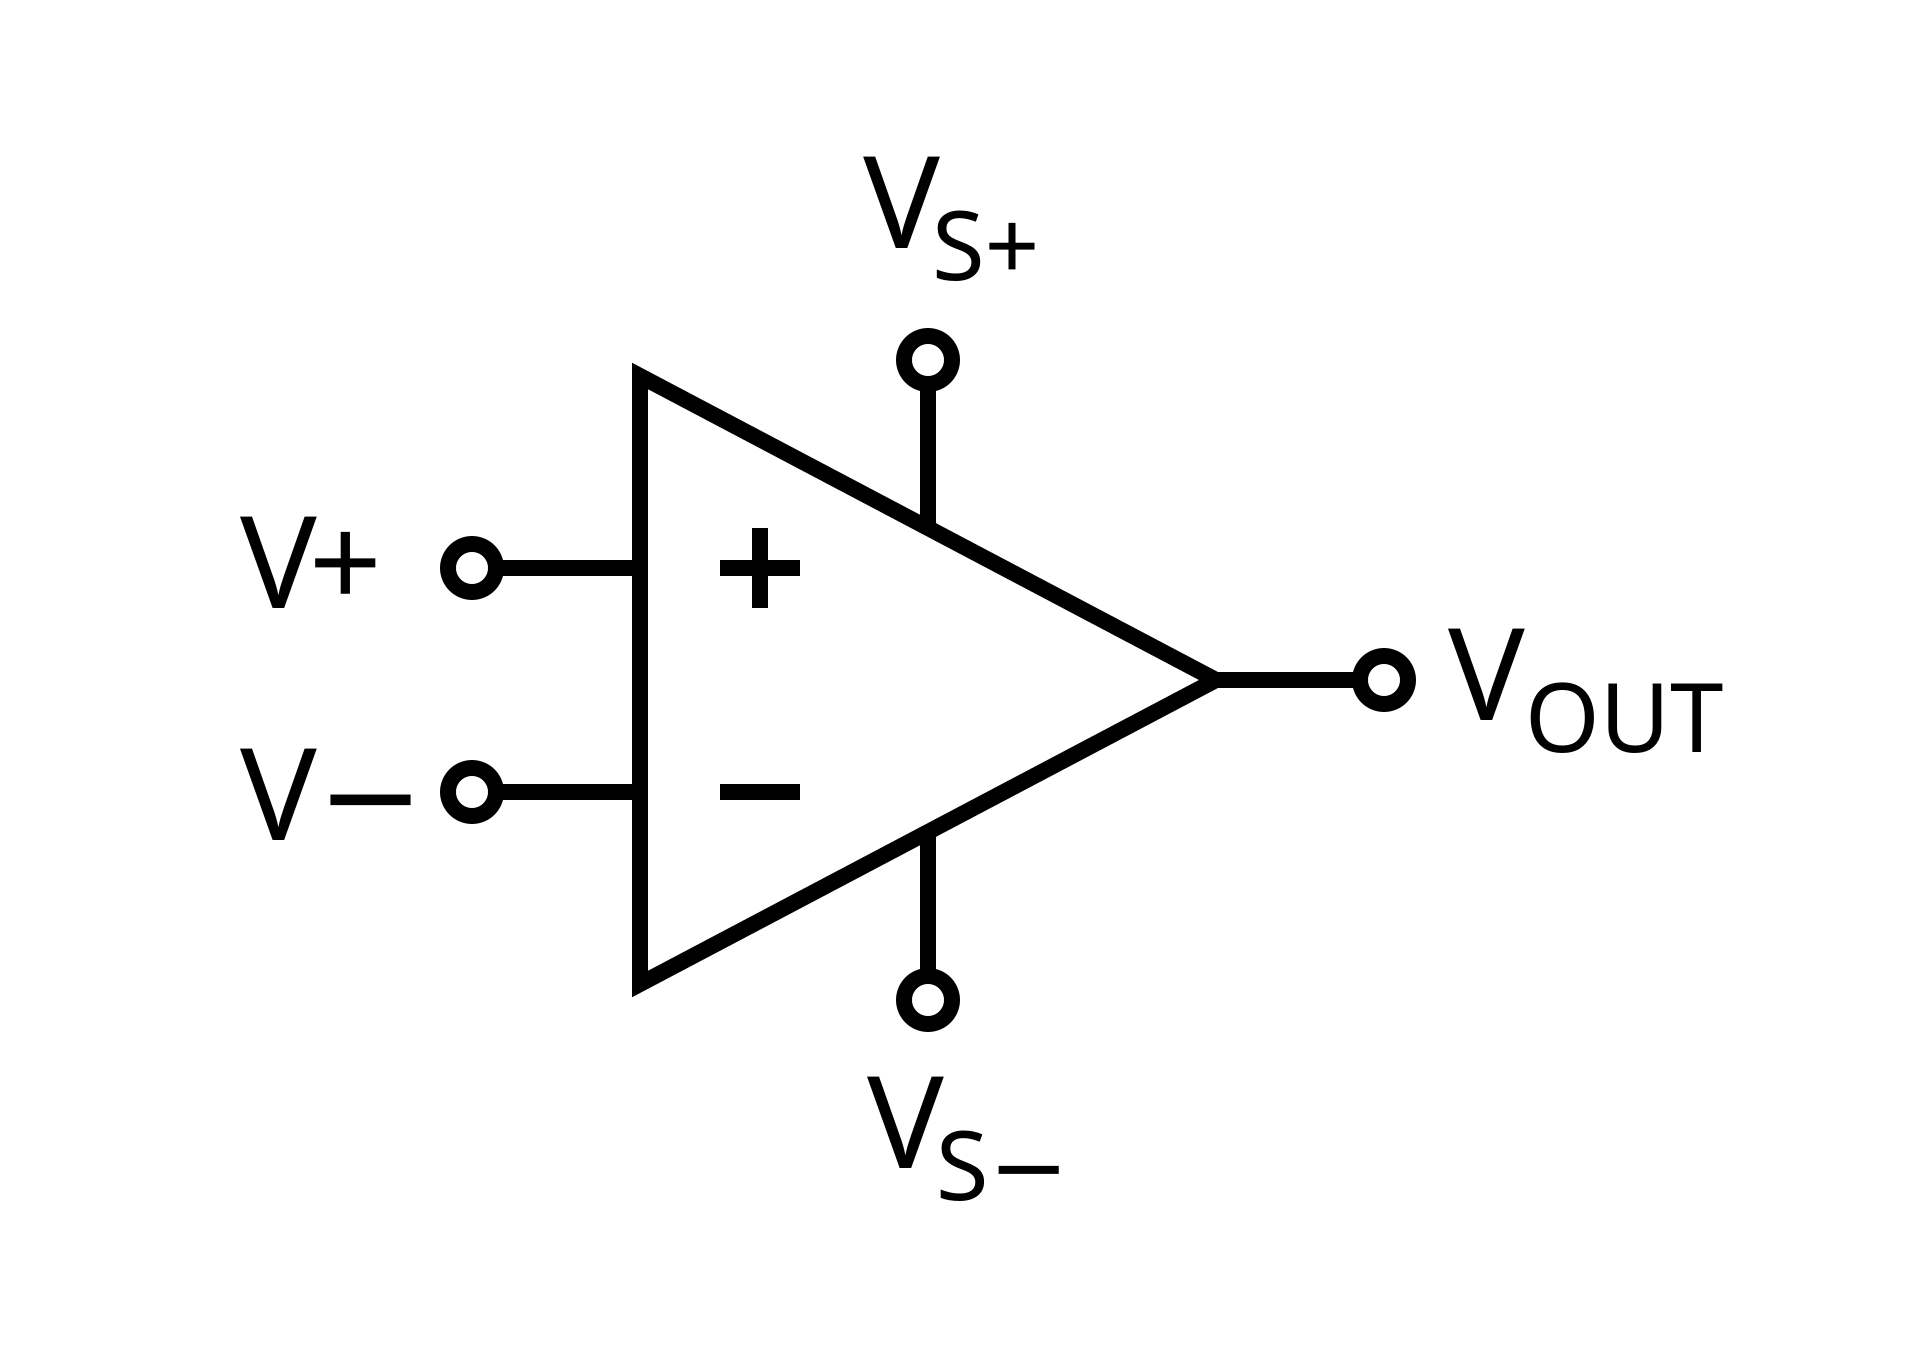
\includegraphics[width=0.3\linewidth]{opamp.png}
    \caption{An operational amplifier (Souce: The Internet)}
\end{figure}
As we can see in the given figure above, an opamp has an inverting input, and a non-inverting input.
The gain of the amplifier is given by
$$A = \frac{V_{out}}{V_+ - V_-}$$
Generally $A$ is extremely large, however an OPAMP cannot produce arbitrarily high voltages. The 
maximum voltage it can produce is decided the power supply connected to it, which is denoted by $V_{S\pm}$.

In this experiment and in most cases in general, we have chosen $V_S = 15 V$. So, the output of the 
OPAMP saturates at $V_S$, and hence, it does not follow the linear gain relation we have mentioned above.

Also, out opAmp of choice in this experiment is the LM741 Operational amplifier. The pinouts of this
IC have been given below.

\begin{figure}[!h]
    \centering
    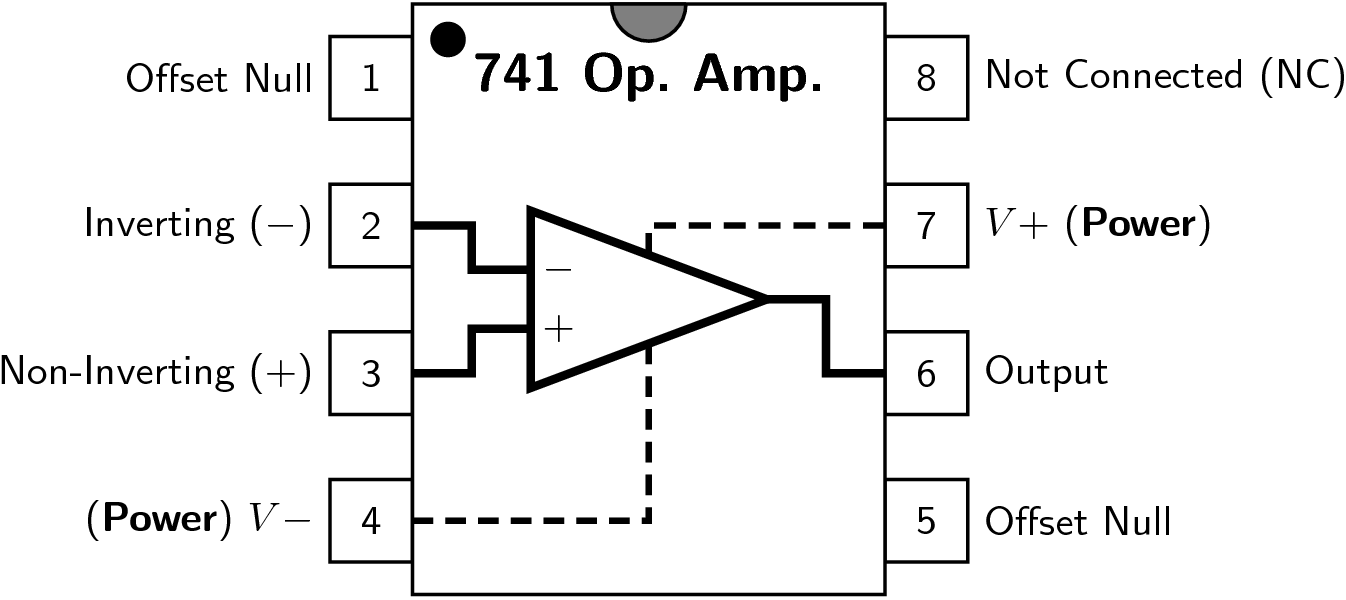
\includegraphics[width=0.3\linewidth]{opampic741.png}
    \caption{LM741 pinouts (Souce: The Internet)}
\end{figure}
\pagebreak
\subsection{Inverting Amplifier}
In this configuration, the output of the OPAMP is of the opposite sign of the input voltage.
The circuit diagram of this configuration is given below.

\begin{figure}[!h]
    \centering
    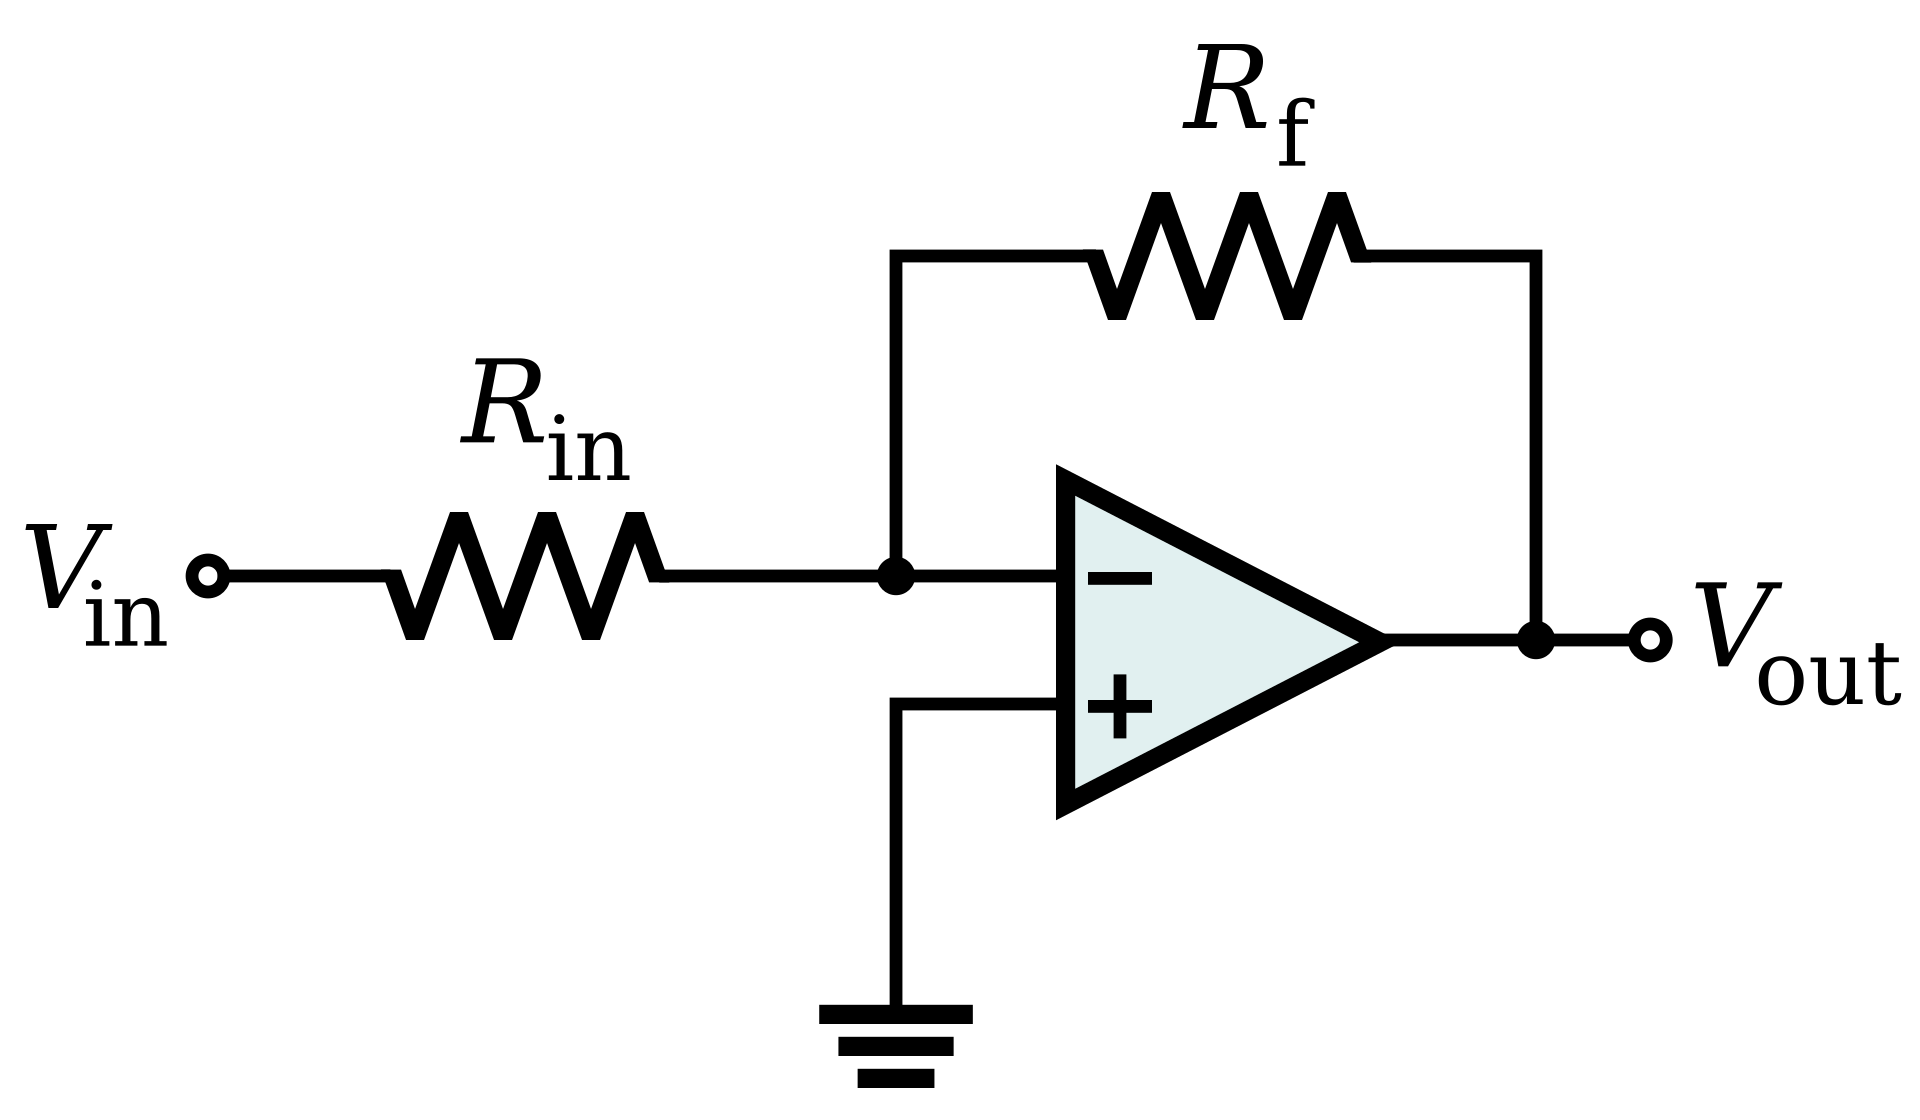
\includegraphics[width=0.6\linewidth]{invertingamp.png}
    \caption{An op amp connected in the inverting amplifier configuration (Source: Internet)}
\end{figure}

In this case, the gain of the amplifier is decided by the two resistors, and is given by the formula
$$A = -\cfrac{R_f}{R_i}$$

The minus sign here is where the "inverting" nature arises, since the input is connected to the inverting
input terminal of the OPAMP.

\subsection{Non Inverting Amplifier}
In this configuration, the output of the OPAMP is of the same sign of the input voltage.
The circuit diagram of this configuration is given below.

\begin{figure}[!h]
    \centering
    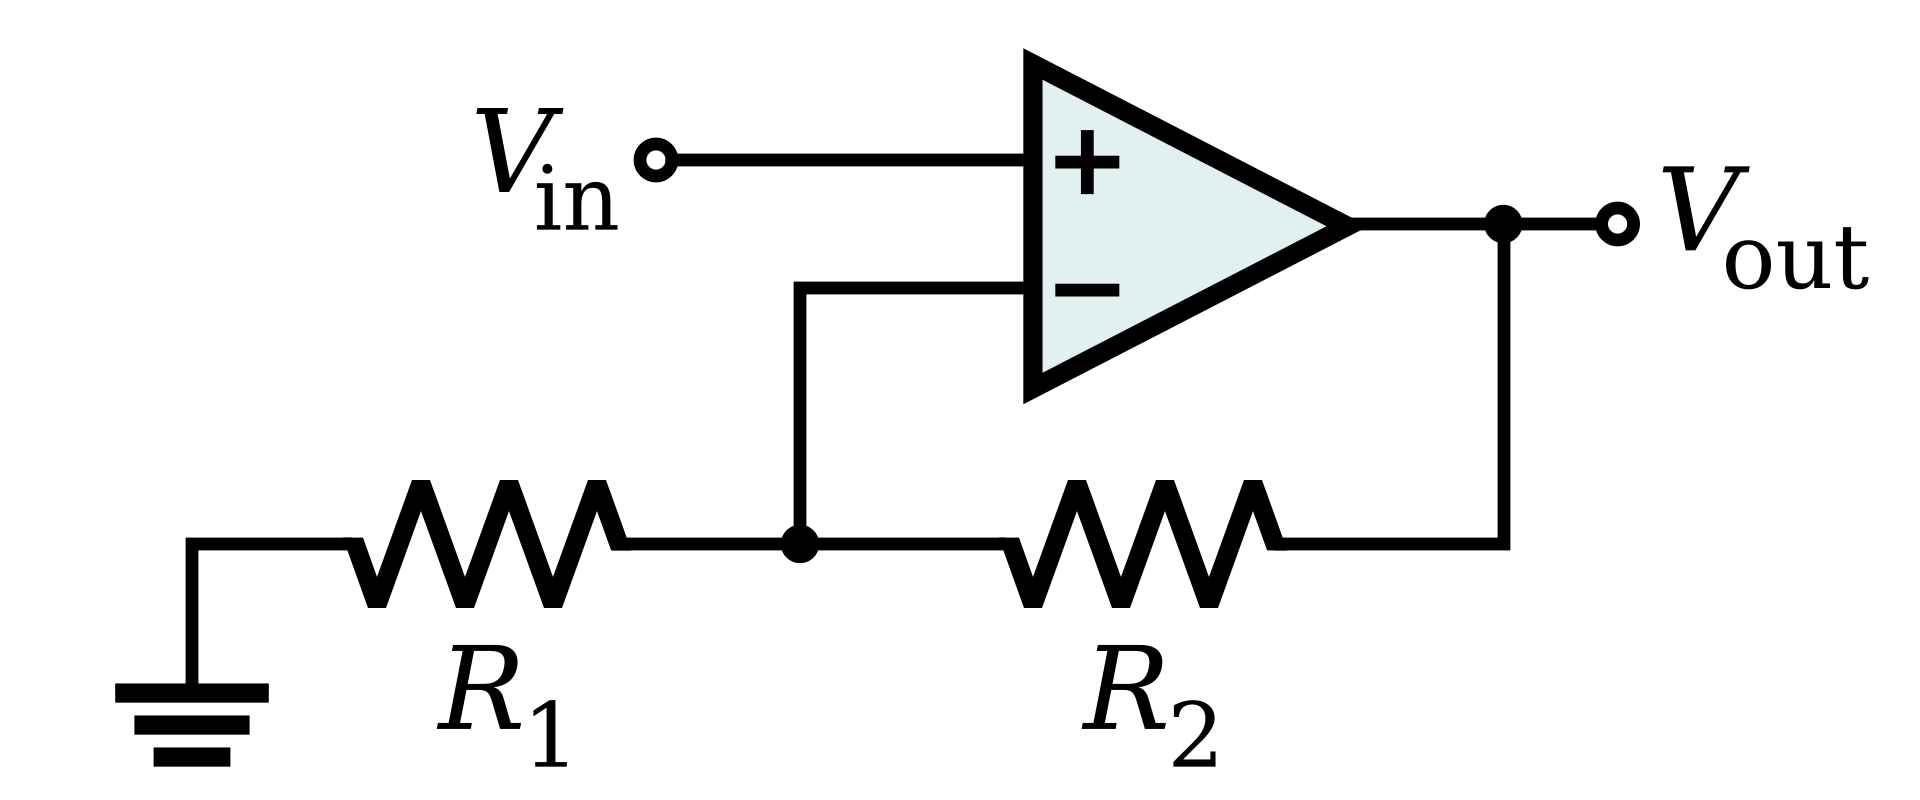
\includegraphics[width=0.6\linewidth]{noninvertingamp.png}
    \caption{An op amp connected in the non-inverting amplifier configuration (Source: Internet)}
\end{figure}

In this case, the gain of the amplifier is decided by the two resistors, and is given by the formula
$$A = 1 + \cfrac{R_2}{R_1}$$

Again, it's non-inverting because this time, the input signal is being fed into the non-inverting terminal
of the OPAMP.
\clearpage
\subsection{Voltage Adder}
In this configuration, the output of the OPAMP is given by a weighted sum of the input voltages, 
with a minus sign, because it's being sent through the inverting terminal of the OPAMP. The
circuit diagram for this configuration is given below.

\begin{figure}[!h]
    \centering
    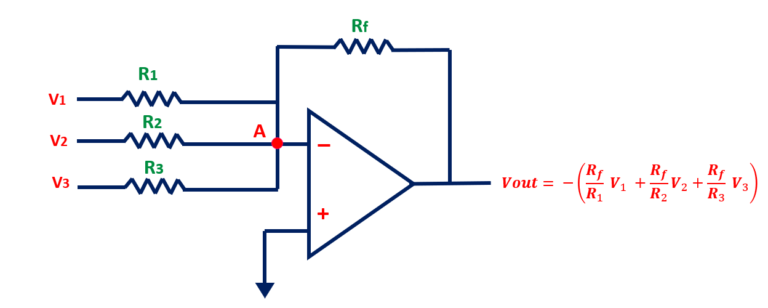
\includegraphics[width=0.7\linewidth]{adder.png}
    \caption{An op amp connected in the voltage adder configuration (Source: Internet)}
\end{figure}

In this configuration, the output of the OPAMP is given by, 
$$V_o = -R_f\left(\cfrac{V_1}{R_1} + \cfrac{V_2}{R_2} + \cfrac{V_3}{R_3}\right)$$
\subsection{Voltage Subtractor}
In this configuration, the output of the OPAMP is given by a weighted difference of the input voltages, 
with a minus sign, because it's being sent through the inverting terminal of the OPAMP. The
circuit diagram for this configuration is given below.

\begin{figure}[!h]
    \centering
    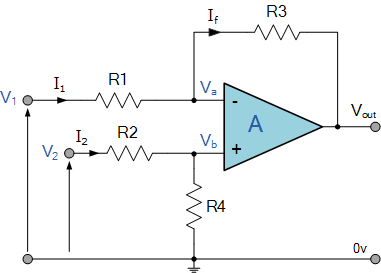
\includegraphics[width=0.4\linewidth]{subtractor.png}
    \caption{An op amp connected in the voltage subtractor configuration (Source: Internet)}
\end{figure}

In this configuration, the output of the OPAMP is given by, 
$$V_o = -R_f\left(\cfrac{V_1}{R_1} - \cfrac{V_2}{R_2}\right)$$

\section{Data and Analysis}
The data tables fot thi experiment have been provided in the supplementary section.
\subsection{Analysis}
huhu
\section{Conclusion}
bado badi bado badi
\section{Sources Of Error}
\begin{enumerate}
    \item Chicken Dak Bungalow
    
\end{enumerate}
\section{Supplementary}
\begin{table}[!ht]
    \centering
    \begin{tabular}{|c|c|c|c|c|c|}
    \hline
        \textbf{-R\_f/R\_i} & \textbf{A(Theo.)} & \textbf{Vi(V)} & \textbf{Vo(V)} & \textbf{A(Expt)} \\ \hline
        -9.8/1 & -9.8 & -0.5 & 4.9 & -9.8 \\ \hline
        -9.8/1 & -9.8 & -0.99 & 9.67 & -9.767676768 \\ \hline
        -9.8/1 & -9.8 & 0.5 & -4.91 & -9.82 \\ \hline
        -9.8/1 & -9.8 & 1 & -9.78 & -9.78 \\ \hline
        -9.8/2.16 & -4.537037037 & 1 & -4.56 & -4.56 \\ \hline
        -9.8/2.16 & -4.537037037 & 0.5 & -2.28 & -4.56 \\ \hline
        -9.8/2.16 & -4.537037037 & -0.99 & 4.49 & -4.535353535 \\ \hline
        -9.8/2.16 & -4.537037037 & -0.5 & 2.27 & -4.54 \\ \hline
        -21.7/9.8 & -2.214285714 & -0.49 & 1.09 & -2.224489796 \\ \hline
        -21.7/9.8 & -2.214285714 & -1 & 2.2 & -2.2 \\ \hline
        -21.7/9.8 & -2.214285714 & 0.49 & -1.09 & -2.224489796 \\ \hline
        -21.7/9.8 & -2.214285714 & 1 & -2.2 & -2.2 \\ \hline
        -2.16/1 & -2.16 & 1 & -2.16 & -2.16 \\ \hline
        -2.16/1 & -2.16 & 0.5 & -1.08 & -2.16 \\ \hline
        -2.16/1 & -2.16 & -1 & 2.17 & -2.17 \\ \hline
        -2.16/1 & -2.16 & -0.5 & 1.08 & -2.16 \\ \hline
        -3.16/1 & -3.16 & -1 & 3.17 & -3.17 \\ \hline
        -3.16/1 & -3.16 & 0.51 & -1.62 & -3.176470588 \\ \hline
        -3.16/1 & -3.16 & 1 & -3.17 & -3.17 \\ \hline
        -3.16/1 & -3.16 & -0.49 & 1.56 & -3.183673469 \\ \hline
    \end{tabular}
    \caption{Inverting Amplifier}
\end{table}
\begin{table}[!ht]
    \centering
    \begin{tabular}{|c|c|c|c|c|c|}
    \hline
        \textbf{1 + R\_f/R\_i} & \textbf{A(Theo.)} & \textbf{Vi(V)} & \textbf{Vo(V)} & \textbf{A(Expt)} \\ \hline
        1+2.16/1 & 3.16 & 1 & 3.17 & 3.17 \\ \hline
        1+2.16/1 & 3.16 & 0.5 & 1.58 & 3.16 \\ \hline
        1+2.16/1 & 3.16 & -1 & -3.15 & 3.15 \\ \hline
        1+2.16/1 & 3.16 & -0.5 & -1.57 & 3.14 \\ \hline
        1+9.08/1 & 10.08 & -0.49 & -5.36 & 10.93877551 \\ \hline
        1+9.08/1 & 10.08 & -1 & -10.82 & 10.82 \\ \hline
        1+9.08/1 & 10.08 & 0.5 & 5.46 & 10.92 \\ \hline
        1+9.08/1 & 10.08 & 1 & 10.9 & 10.9 \\ \hline
        1+21.7/9.8 & 3.214285714 & 1 & 3.2 & 3.2 \\ \hline
        1+21.7/9.8 & 3.214285714 & 0.5 & 1.61 & 3.22 \\ \hline
        1+21.7/9.8 & 3.214285714 & -1 & -3.19 & 3.19 \\ \hline
        1+21.7/9.8 & 3.214285714 & -0.5 & -1.6 & 3.2 \\ \hline
        1+9.8/2.16 & 5.537037037 & -0.5 & -2.75 & 5.5 \\ \hline
        1+9.8/2.16 & 5.537037037 & -0.99 & -5.48 & 5.535353535 \\ \hline
        1+9.8/2.16 & 5.537037037 & 0.5 & 2.77 & 5.54 \\ \hline
        1+9.8/2.16 & 5.537037037 & 1 & 5.53 & 5.53 \\ \hline
        1+3.16 & 4.16 & 0.99 & 4.2 & 4.242424242 \\ \hline
        1+3.16 & 4.16 & 0.5 & 2.11 & 4.22 \\ \hline
        1+3.16 & 4.16 & -0.99 & -4.16 & 4.202020202 \\ \hline
        1+3.16 & 4.16 & -0.49 & -2.04 & 4.163265306 \\ \hline
    \end{tabular}
    \caption{Non-Inverting Amplifier}
\end{table}
\begin{table}[!ht]
    \centering
    \begin{tabular}{|c|c|c|c|c|c|c|}
    \hline
        \textbf{SL no.} & \textbf{V1(V)} & \textbf{V2(V)} & \textbf{V3(V)} & \textbf{Column 1} & \textbf{Vo(meas)} & \textbf{Vo(Theo)} \\ \hline
        1 & 4.93 & 2.01 & 1.07 & 8.16 & -8.16 & 8.01 \\ \hline
        2 & 5.91 & 2.42 & 1.28 & 9.8 & -9.8 & 9.61 \\ \hline
        3 & 2.4 & 1.18 & 0.56 & 4.2 & -4.2 & 4.14 \\ \hline
        4 & 3.94 & 1.58 & 0.86 & 6.5 & -6.5 & 6.38 \\ \hline
        5 & 4 & 1.83 & 1.16 & 7.13 & -7.13 & 6.99 \\ \hline
        6 & 3.28 & 1.45 & 0.8 & 5.63 & -5.63 & 5.53 \\ \hline
        7 & 3.34 & 1.64 & 0.77 & 5.86 & -5.86 & 5.75 \\ \hline
        8 & 5.12 & 2.57 & 1.06 & 8.93 & -8.93 & 8.75 \\ \hline
        9 & 4.49 & 2.2 & 1.04 & 7.88 & -7.88 & 7.73 \\ \hline
        10 & 5.7 & 2.13 & 0.89 & 8.92 & -8.92 & 8.72 \\ \hline
    \end{tabular}
    \caption{Voltage Adder}
\end{table}
\begin{table}[!ht]
    \centering
    \begin{tabular}{|c|c|c|c|c|}
    \hline
        \textbf{SL. no.} & \textbf{V1(V)} & \textbf{V2(V)} & \textbf{Vo(Meas)} & \textbf{Vo(Theo)} \\ \hline
        1 & 0.15 & 1.04 & 0.91 & 0.89 \\ \hline
        2 & 0.26 & 1.04 & 0.82 & 0.78 \\ \hline
        3 & 0.39 & 1.04 & 0.64 & 0.65 \\ \hline
        4 & 1.12 & 3 & 1.97 & 1.88 \\ \hline
        5 & 1.39 & 3.11 & 1.81 & 1.72 \\ \hline
        6 & 1.59 & 4.07 & 2.6 & 2.48 \\ \hline
        7 & 0.86 & 3.55 & 2.78 & 2.69 \\ \hline
        8 & 3.02 & 5.98 & 3.15 & 2.96 \\ \hline
        9 & 1.41 & 5.8 & 4.54 & 4.39 \\ \hline
        10 & 1.08 & 4.42 & 3.46 & 3.34 \\ \hline
        11 & 5.31 & 6.2 & 1.14 & 0.89 \\ \hline
        12 & 3.69 & 4.56 & 1.05 & 0.87 \\ \hline
        13 & 3.34 & 4.46 & 1.29 & 1.12 \\ \hline
        14 & 4.13 & 3.25 & -0.71 & -0.88 \\ \hline
        15 & 4.85 & 3.81 & -0.83 & -1.04 \\ \hline
        16 & 5.79 & 4.73 & -0.82 & -1.06 \\ \hline
        17 & 3.36 & 1.6 & -1.64 & -1.76 \\ \hline
        18 & 3.5 & 2.25 & -1.11 & -1.25 \\ \hline
        19 & 5.32 & 1.15 & -4.01 & -4.17 \\ \hline
        20 & 5.13 & 1.11 & -3.87 & -4.02 \\ \hline
        21 & 3.05 & 0.66 & -2.3 & -2.39 \\ \hline
        22 & 2.19 & 0.47 & -1.65 & -1.72 \\ \hline
        23 & 1.43 & 0.3 & -1.07 & -1.13 \\ \hline
    \end{tabular}
    \caption{Voltage Subtractor}
\end{table}
\end{document}
